In this section we evaluate the performance of our work-stealing framework built on SALSA pools. 
We describe the experiment setup in Section~\ref{sec:exp-setup}, we show the overall system performance in Section~\ref{sec:eval-performance} and study the influence of various SALSA techniques in Section~\ref{sec:eval-techniques}.

\subsection {Experiment Setup}
\label{sec:exp-setup}
The implementation of the work-stealing framework used in our evaluation does not include the linearizability mechanism described in~\ref{sec:correctness}. We believe that this mechanism has negligible effect on performance; moreover, in our experiment they would not have been invoked because the pool is never empty. We compare the following task pool implementations:
\begin {itemize}
\item
{\bf SALSA} -- our work-stealing framework with SCPools implemented by SALSA.
\item
{\bf SALSA+CAS} -- our work-stealing framework with SCPools implemented by a simplistic SALSA variation, in which every {\bf consume()} and {\bf steal()} operation tries to take a single task using CAS. In essence, SALSA+CAS removes the effects of SALSA's low-synchronization fast-path and per-chunk stealing. 
Note that disabling per-chunk stealing in SALSA annuls the idea of chunk ownership, hence, disables its low-synchronization fast-path as well. 
\item
{\bf ConcBag} -- an algorithm similar to the lock-free Concurrent Bags algorithm~\cite{Sundell:2011:LAC:1989493.1989550}. 
It is worth noting that the original algorithm was optimized for the scenario where the same process is both a producer and a consumer (in essence producing tasks to itself), which we do not consider in this paper; in our system no thread acts as both a producer and a consumer, therefore every consume operation steals a task from some producer.
We did not have access to the original code, and therefore reimplemented the algorithm in our framework. Our implementation is faithful to the algorithm in the paper, except in using a simpler and faster underlined linked list algorithm. All engineering decisions were made to maximize performance. 
\item
{\bf WS-MSQ} -- our work-stealing framework with SCPools implemented by Michael-Scott non-blocking queue~\cite{Michael:1996:SFP:248052.248106}. Both {\bf consume()} and {\bf steal()} operations invoke the {\bf dequeue()} function. 
\item
{\bf WS-LIFO} -- our work-stealing framework with SCPool implemented by Michael's LIFO stack~\cite{Michael:2004:HPS:987524.987595}. 
\end {itemize} 

We did not experiment with additional FIFO and LIFO queue implementations, because, as shown in~\cite{Sundell:2011:LAC:1989493.1989550}, their performance is of the same order of magnitude as the Michael-Scott queue. 
Similarly, we did not evaluate {CAF\'E}\cite{Basin:2011:CST:2075029.2075087} pools because their performance is similar to that of WS-MSQ~\cite{Basin:Thesis:2011}, or ED-Pools~\cite{Afek:2010:SPP:1885276.1885295}, which have been shown to scale poorly in multi-processor architectures~\cite{Basin:Thesis:2011,Sundell:2011:LAC:1989493.1989550}. 

All the pools are implemented in C++ and compiled with \texttt{-O2} optimization level. 
In order to minimize scalability issues related to allocations, we use \texttt{jemalloc} allocator~\cite{citeulike:4951109}, which has been shown to be highly scalable in multi-threaded environments\footnote{\url{http://www.facebook.com/notes/facebook-engineering/scalable-memory-allocation-using-jemalloc/480222803919}}.
Chunks of SALSA and SALSA+CAS contain $1000$ tasks, and chunks of ConcBag contain $128$ tasks, which were the respective optimal values for each algorithm (see Appendix \ref{appendix:chunk-size}). 

We use a synthetic benchmark where 1) each producer works in a loop of inserting dummy items; 2) each consumer works in a loop of retrieving dummy items. Each data point shown is an average of $5$ runs, each with a duration of $20$ seconds. 
The tests are run on a dedicated shared memory NUMA server with $8$ Quad Core AMD $2.3$GHz processors and $16$GB of memory attached to each processor. 

\subsection{System Throughput}
\label{sec:eval-performance}

\begin{figure}[htb]
	\centering
  \subfigure [\scriptsize{System throughput -- N producers, N consumers.}] {
    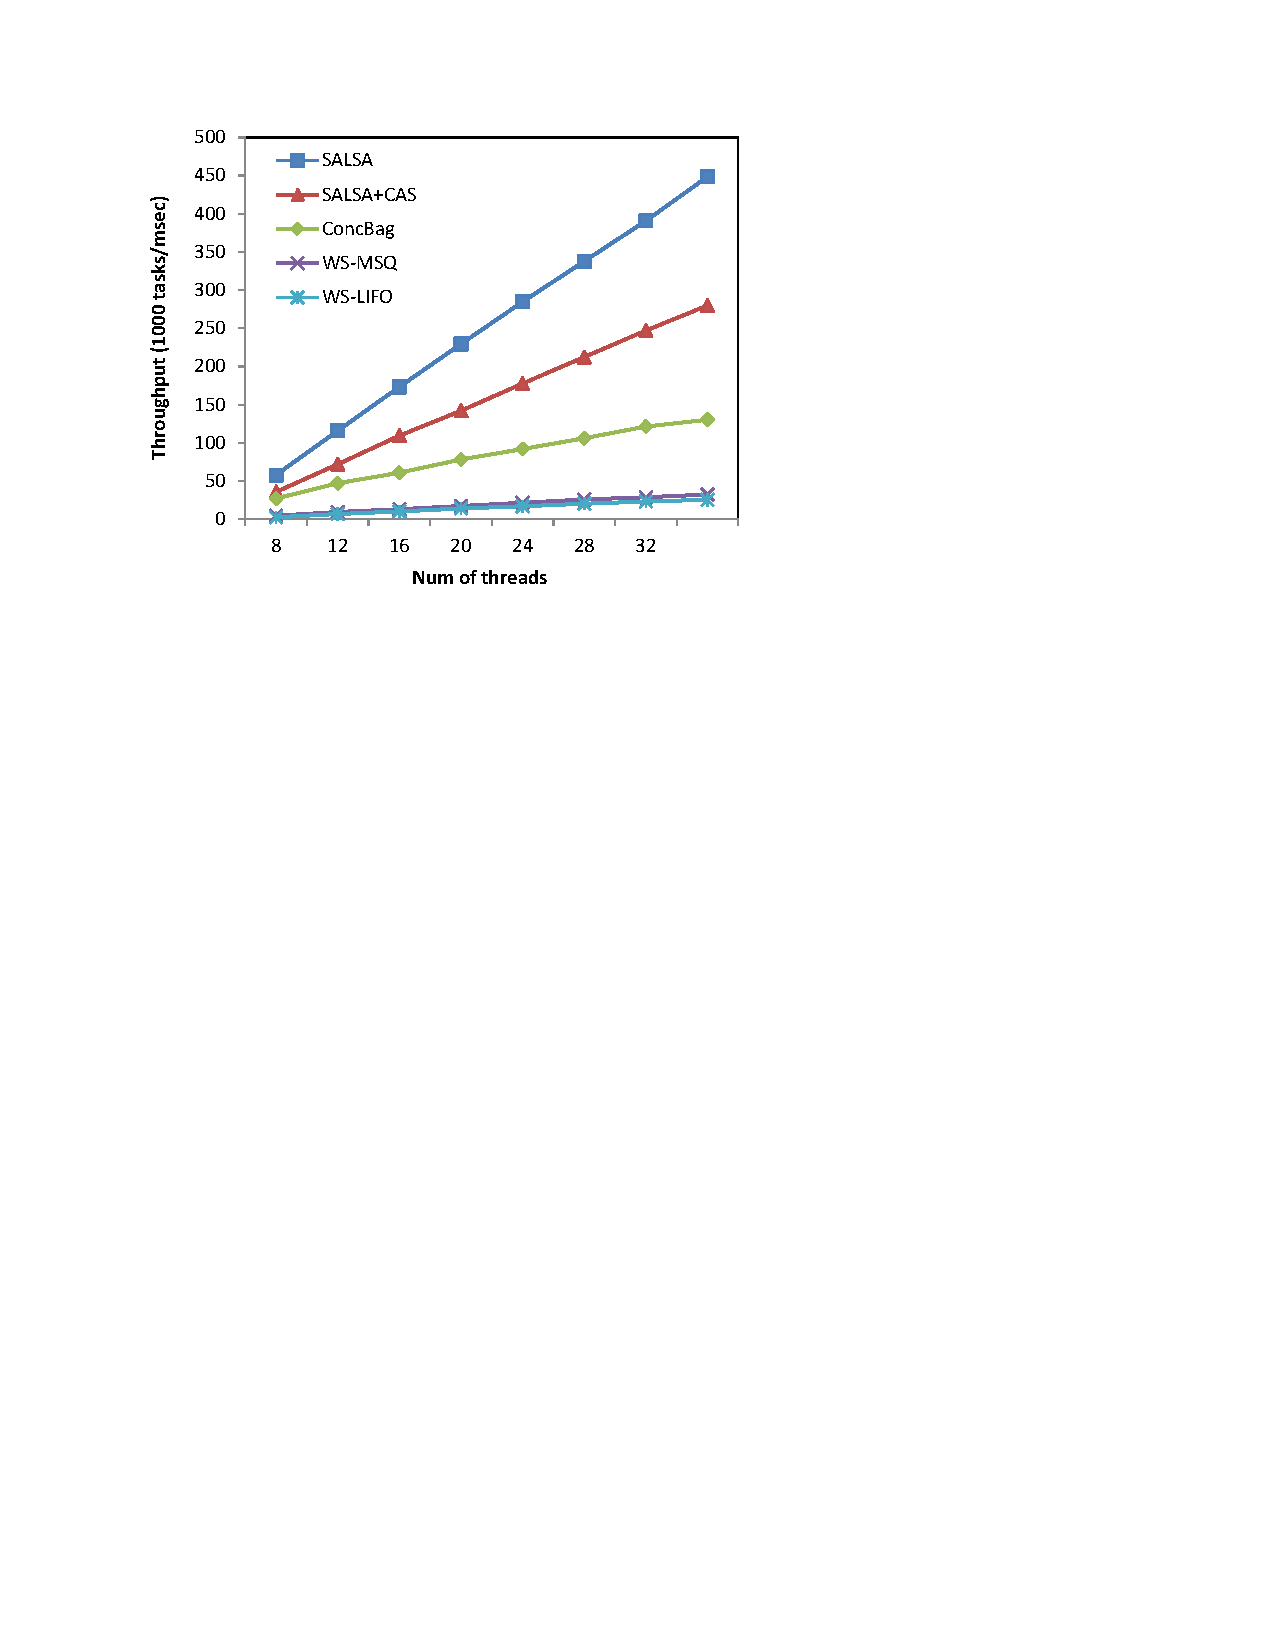
\includegraphics[width=0.45\textwidth]{figures/n-n-throughput}
    \label{fig:n-n-throughput}
  }
  \subfigure [\scriptsize{System throughput -- variable producers-consumers ratio.}] {
    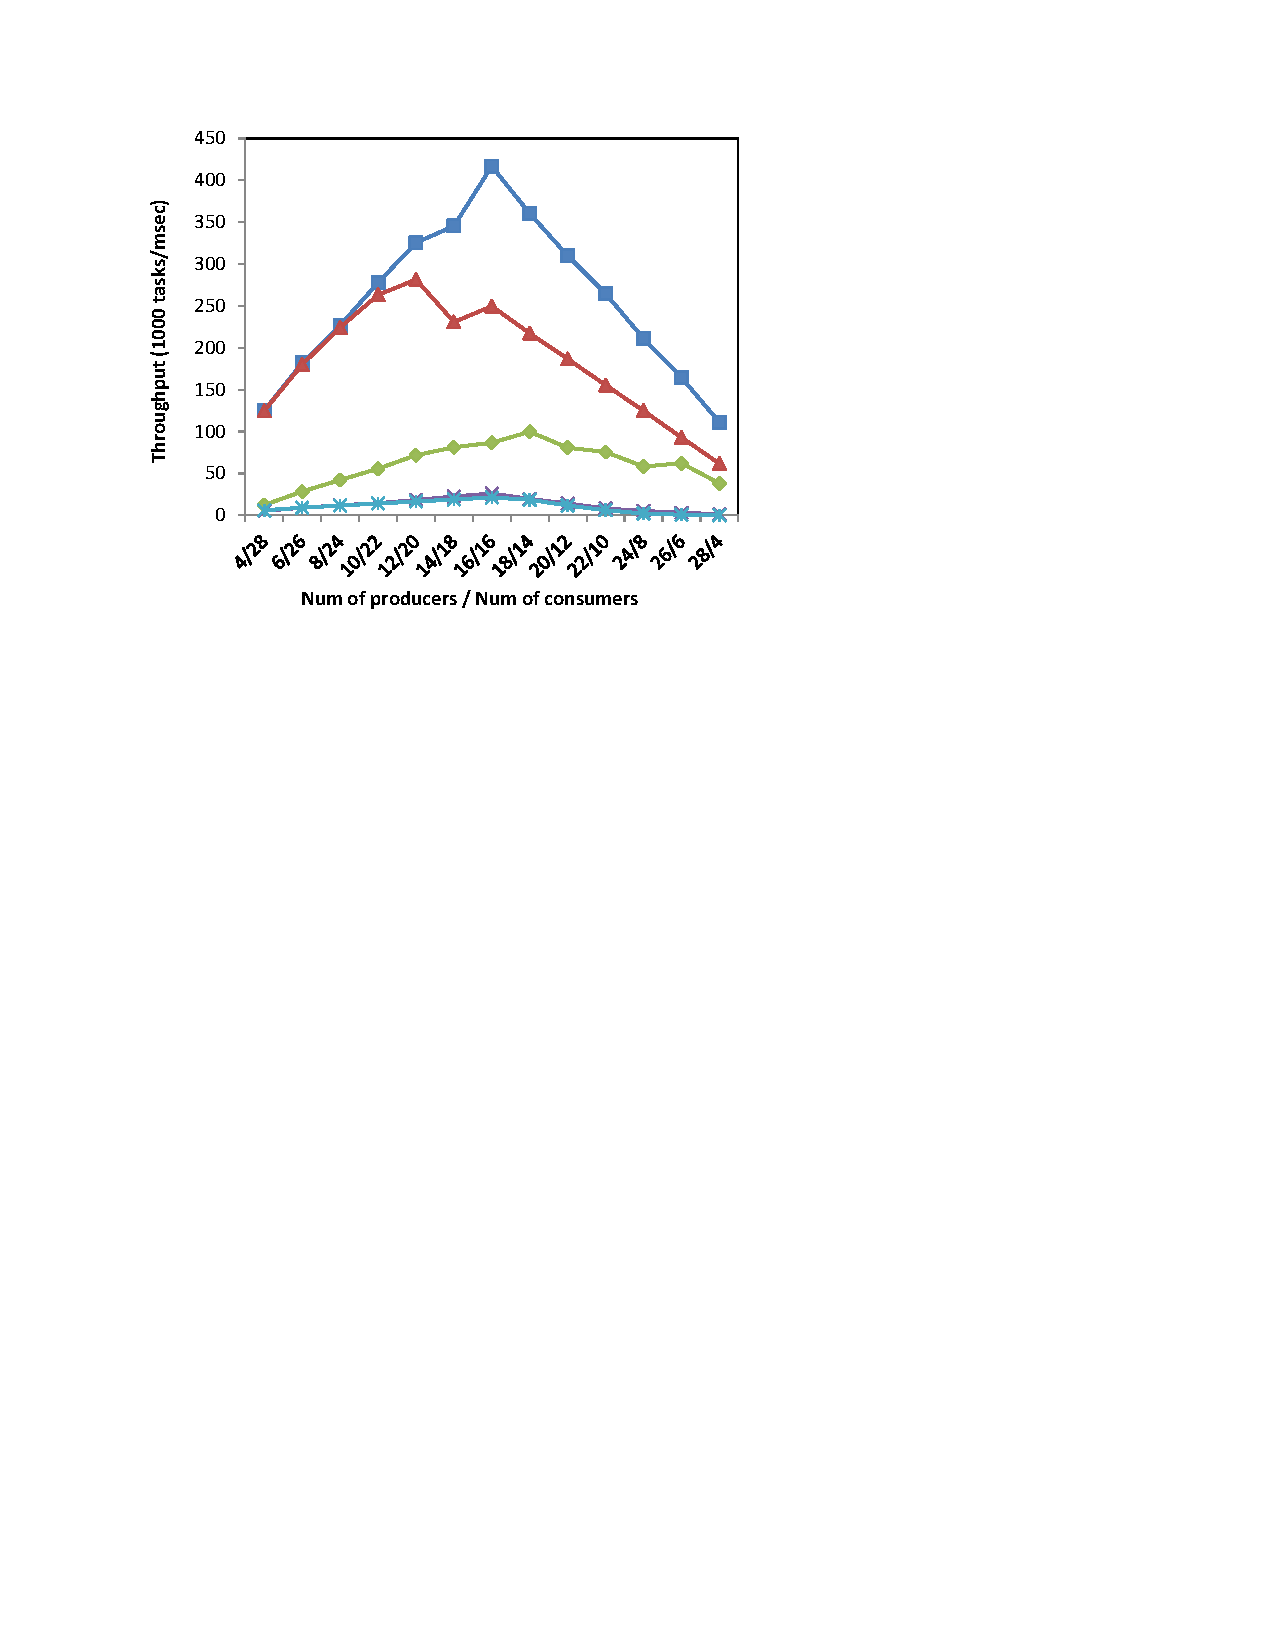
\includegraphics[width=0.45\textwidth]{figures/prod-cons-fig}
    \label{fig:prod-cons-fig}
  }
	\caption{\footnotesize{System throughput for various ratios of producers and consumers. SALSA scales linearly with the number of threads -- in the $16/16$ workload, it is $\times20$ faster than WS-MSQ and WS-LIFO, and more than $\times5$ faster than Concurrent Bags. In tests with equal numbers of producers and consumers, the differences among work-stealing alternatives are mainly explained by the consume operation efficiency, since stealing rate is low and hardly influences performance. In Concurrent Bags every {\bf consume()} operation implies stealing, which causes its sub-linear scalability.
}}
	\label{fig:throughput}
\end{figure}

Figure~\ref{fig:throughput} demonstrates system throughput of the compared algorithms for workloads with various numbers of producers and consumers. 
Figure~\ref{fig:n-n-throughput} shows throughput dynamics when the number of producers is equal to the number of consumers. SALSA \emph{scales linearly} as the number of threads grows to $32$ (the number of physical cores in the system), and it clearly outperforms all other competitors. In the $16/16$ workload, SALSA is $\times20$ faster than WS-MSQ and WS-LIFO, and more than $\times5$ faster than Concurrent Bags. 

We note that the performance trend of ConcBags in our measurements differs from the results presented by Sundell et al.~\cite{Sundell:2011:LAC:1989493.1989550}. 
While in the original paper, their throughput \emph{drops} by a factor of $3$ when the number of threads increases from $4$ to $24$, in our tests, the performance of ConcBags \emph{increases} with the number of threads. The reasons for the better scalability of our implementation compared of the original one can be related to the use of different memory allocators, hardware architectures, and engineering optimizations. %In any case, both implementations provide the performance of tens of thousands of task retrievals in msec for multiple producers and consumers. 

The stealing rate in workloads with equal numbers of producers and consumers remains low; graphs showing these results are omitted due to space limitations. The performance differences are therefore due to the efficiency of the {\bf consume()} operation. 
For example, SALSA is $\times1.7$ faster than SALSA+CAS thanks to the fast-path consumption technique, which does not use strong atomic operations. The impact of CAS operations is fairly modest, however, since they seldom compete.
In contrast, in ConcBags, which is not based on per-consumer pools, every {\bf consume()} operation implies stealing, which causes contention among consumers, leading to sub-linear scalability.

Figure~\ref{fig:prod-cons-fig} shows system throughput of the algorithms for various ratios of producers and consumers. 
Our algorithm achieves maximal throughput for the equal number of producers and consumers because neither of them is a system bottleneck.
SALSA outperforms other alternatives for all possible producer-consumer ratios. 

\begin{figure}[htb]
	\centering
  \subfigure [\scriptsize{System throughput -- 1 Producer, N consumers.}] {
    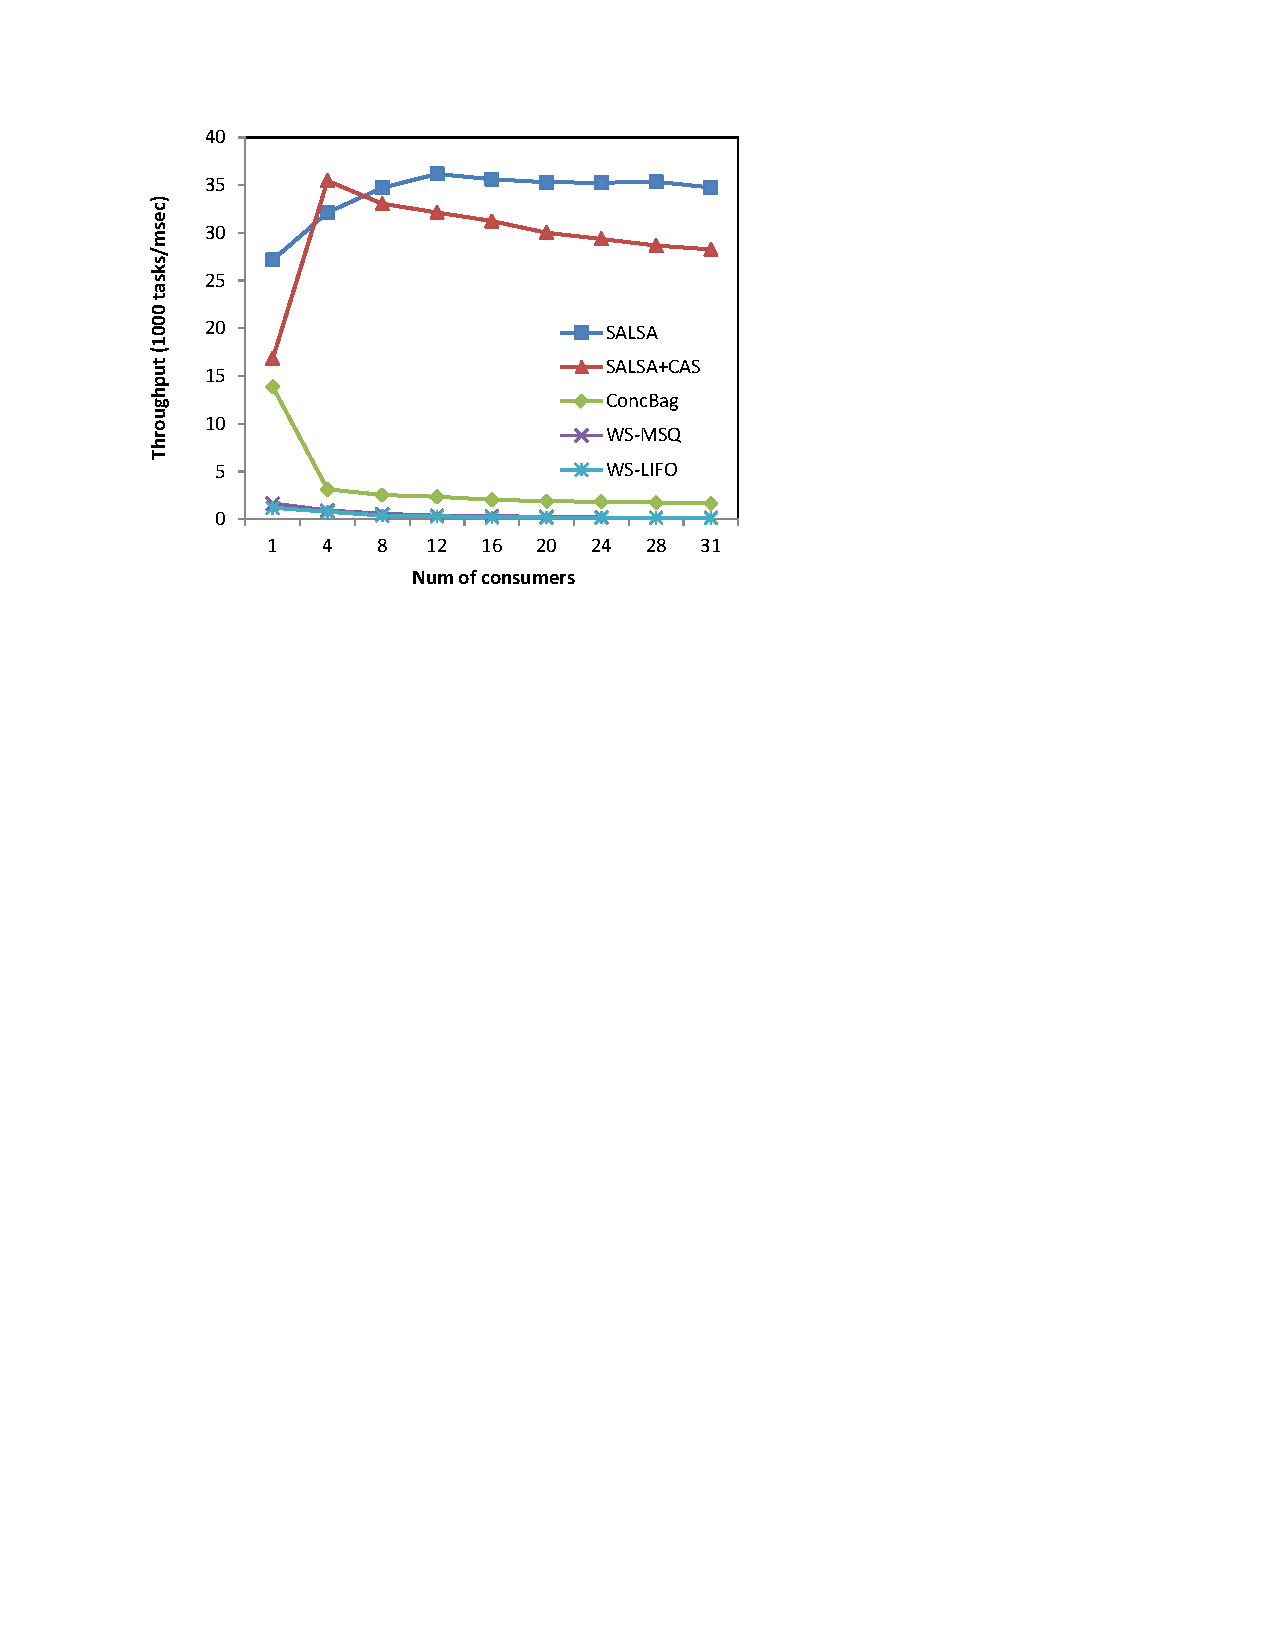
\includegraphics[width=0.45\textwidth]{figures/1-n-throughput}
    \label{fig:1-n-throughput}
  }
  \subfigure [\scriptsize{CAS operations per task retrieval -- 1 Producer, N consumers.}] {
    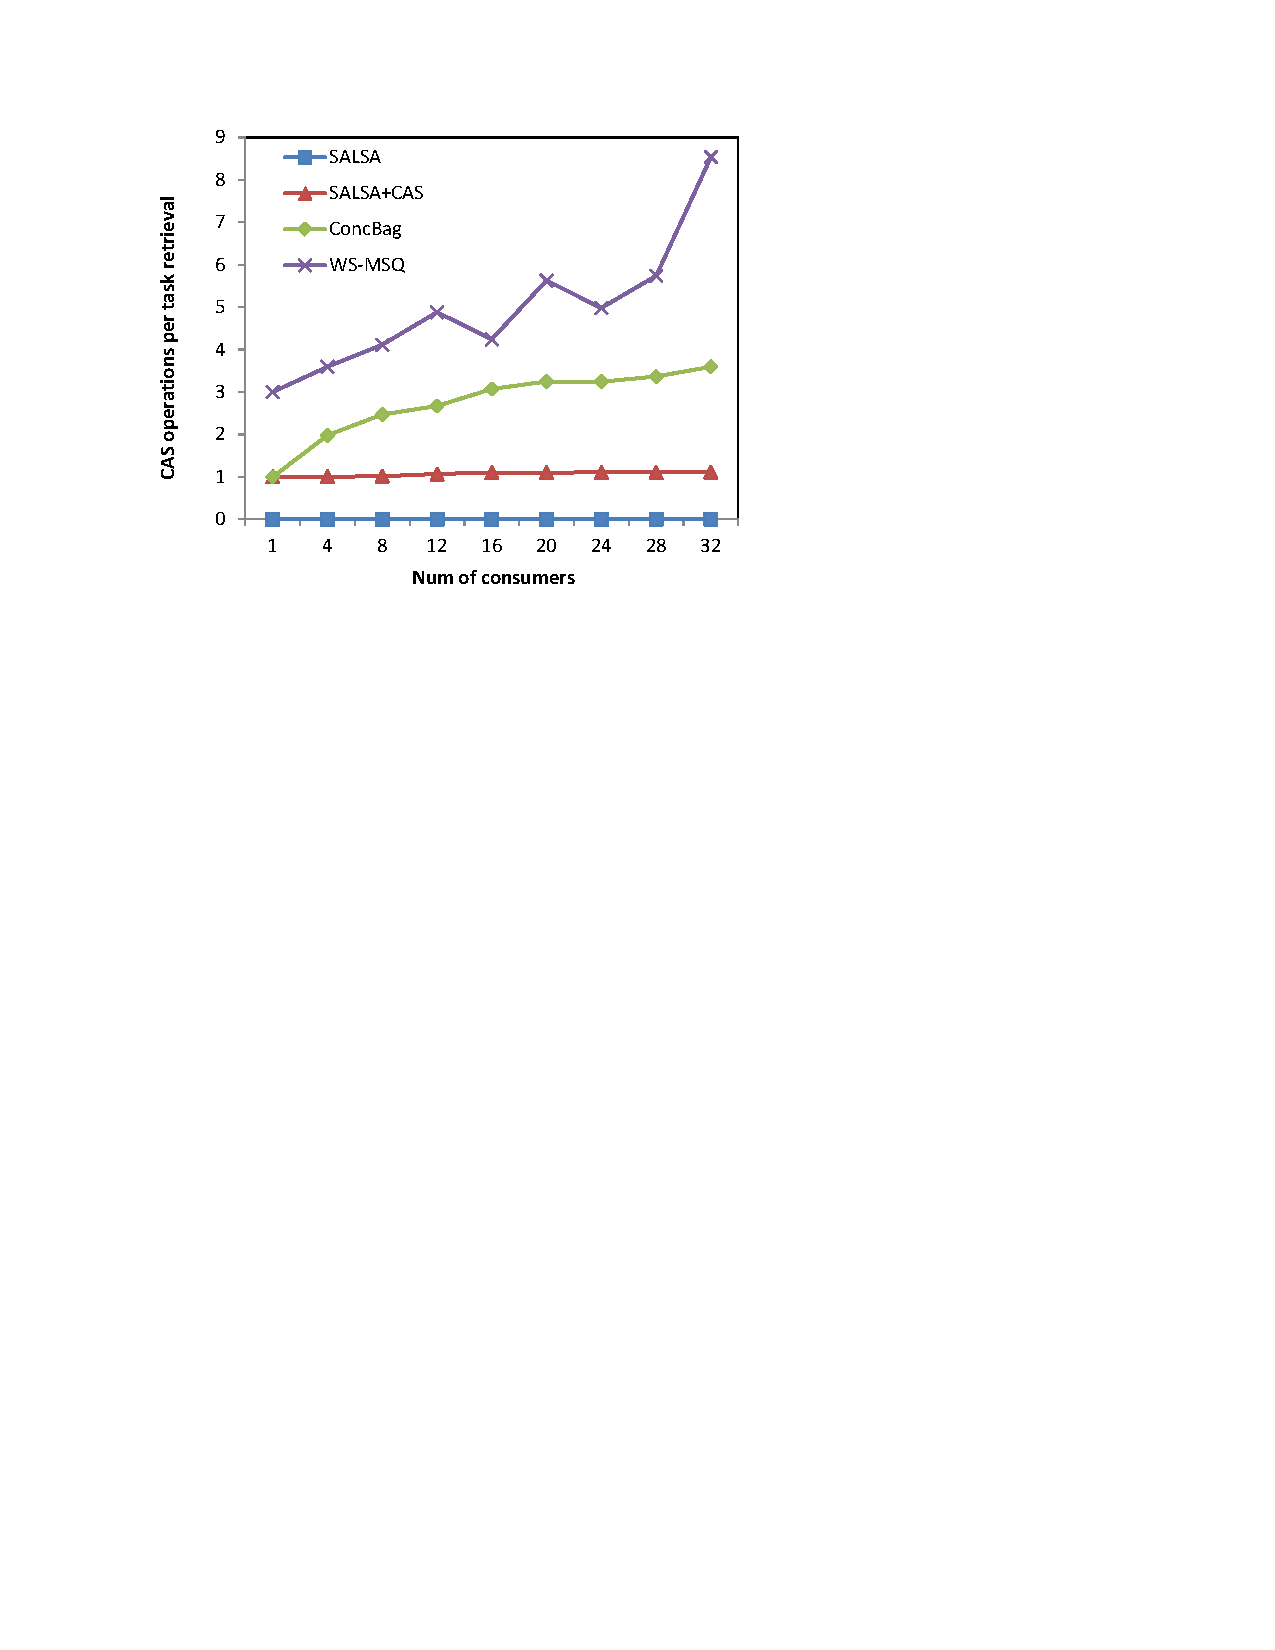
\includegraphics[width=0.45\textwidth]{figures/1-n-cas}
    \label{fig:1-n-cas}
  }
	\caption{\footnotesize{System behavior in workloads with a single producer and multiple consumers. 
	Both SALSA and SALSA+CAS efficiency balance the load in this scenario. The throughput of other algorithms drops by a factor of $10$ due to increased contention among consumers trying to steal tasks from the same pool.}}
	\label{fig:1-n-perf}
\end{figure}

We next evaluate the behavior of the pools in scenarios with a single producer and multiple consumers. 
Figure~\ref{fig:1-n-throughput} shows that for both SALSA and SALSA+CAS the performance does not drop as more consumers are added. In contrast, the throughput of other algorithms drops by the factor of $10$ when the number of consumers rises from $1$ to $32$. 
This degradation is caused by the increased contention among consumers that try to steal tasks from the same pool, as evident from Figure~\ref{fig:1-n-cas}, which shows the average number of CAS operations per task transfer (by both producers and consumers). As we shall see in the next section, SALSA+CAS's low contention is achieved thanks to the producer-based balancing described in Section~\ref{alg-pools}, and SALSA achieves significantly better throughput thanks to chunk-based stealing.

\subsection{Evaluation of SALSA Techniques}
\label{sec:eval-techniques}
\begin{figure}[htb]
	\centering
  \subfigure [\scriptsize{System throughput -- 1 Producer, N consumers.}] {
    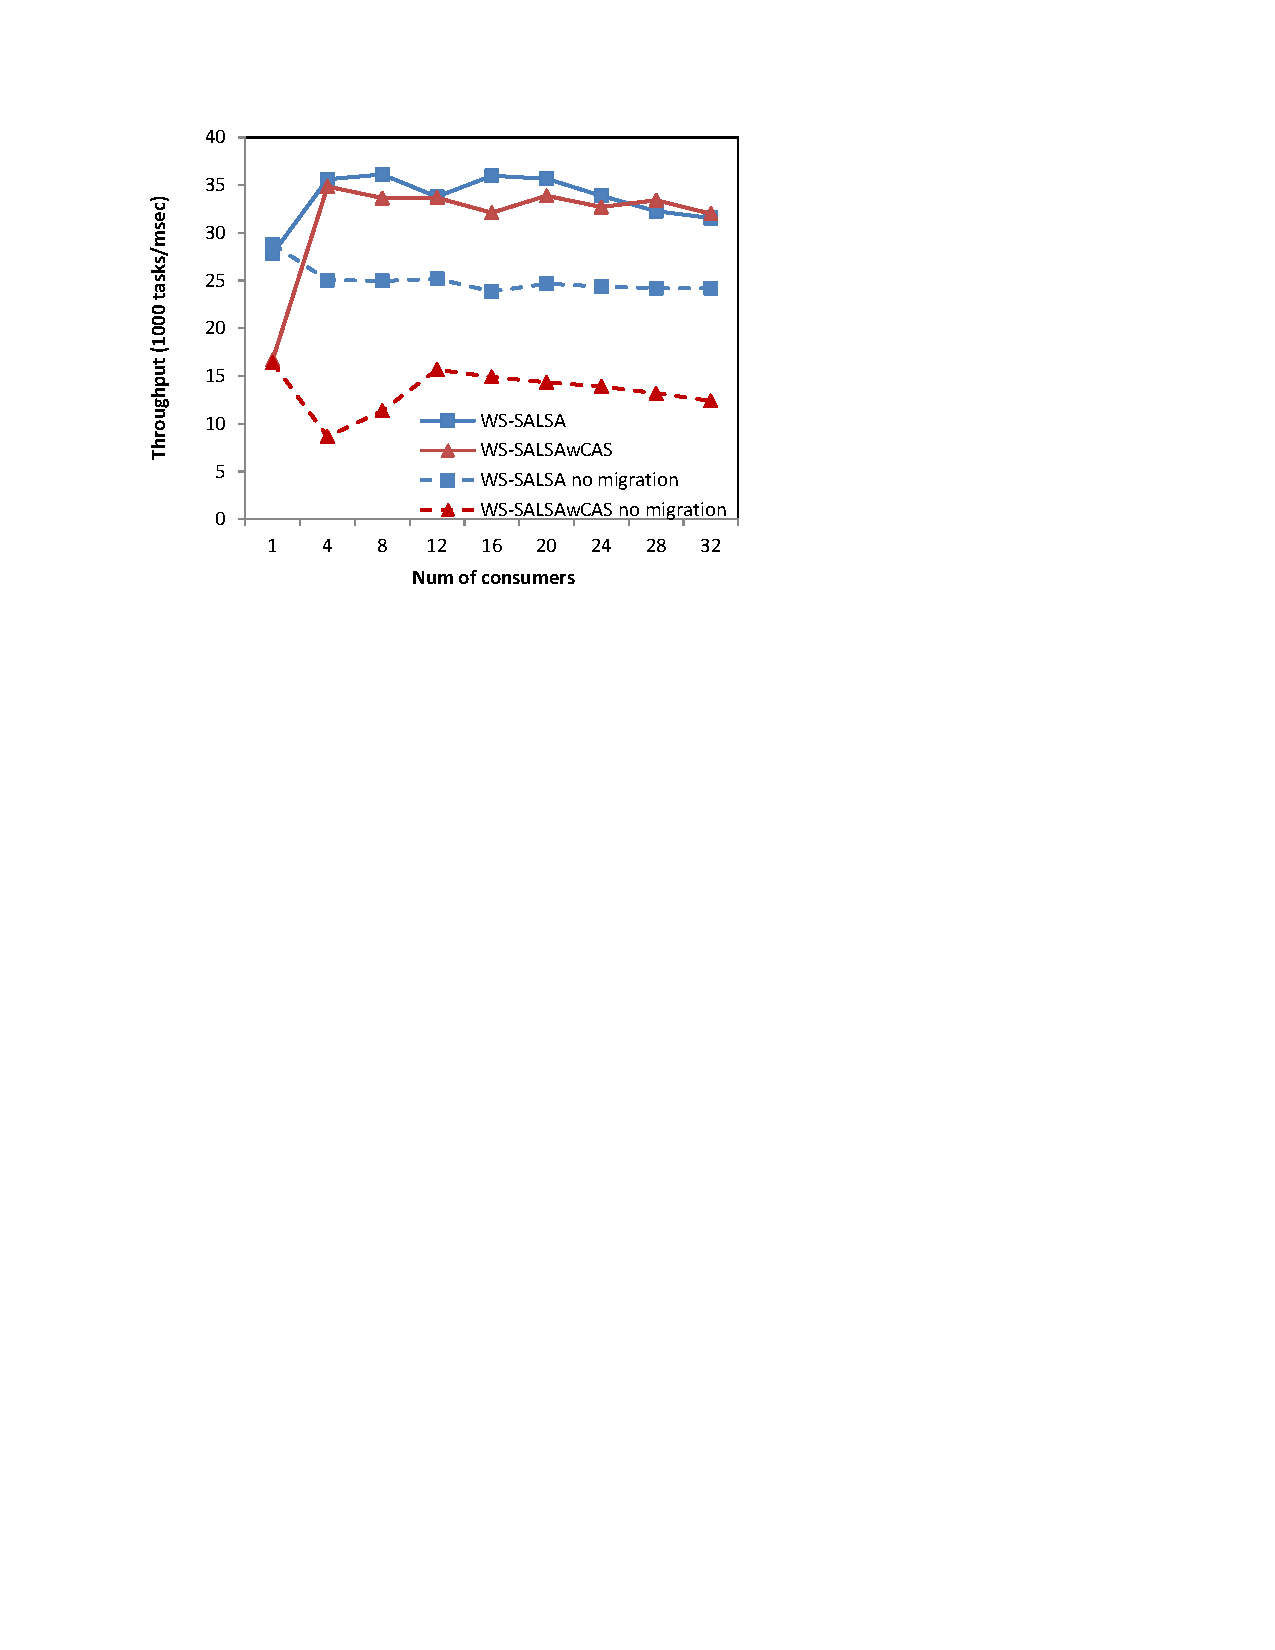
\includegraphics[width=0.45\textwidth]{figures/1-n-salsa}
    \label{fig:1-n-salsa-perf}
  }
  \subfigure [\scriptsize{System throughput as a function of stalled threads ($16/16$ workload). Black dashed lines show the theoretical throughput degradation proportional to the number of stalled threads.}] {
    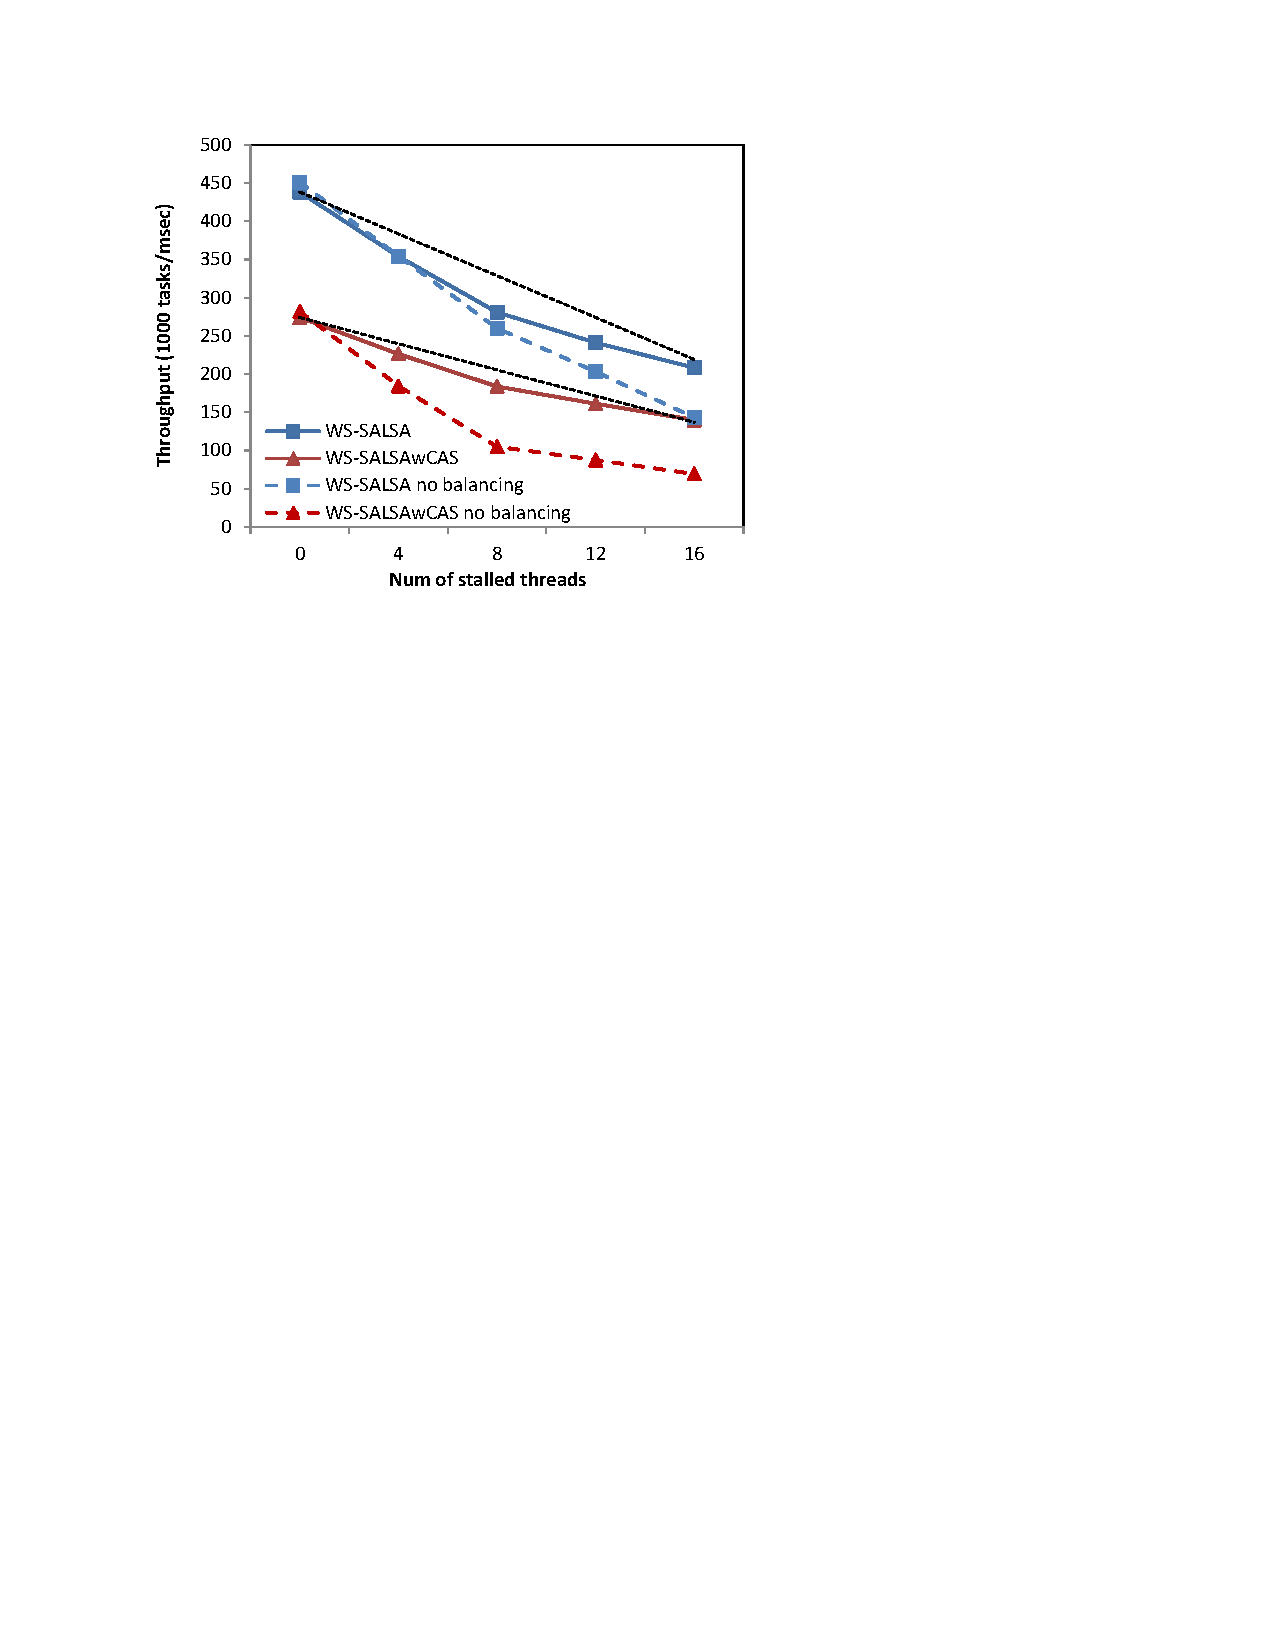
\includegraphics[width=0.45\textwidth]{figures/stalled-threads}
    \label{fig:stalled-threads}
  }
	\caption{\footnotesize{The effects of chunk-based stealing and producer-based balancing on system throughput in imbalanced scenarios. Producer-based balancing contributes to the robustness of the framework by reducing stealing. With no balancing, chunk-based stealing becomes important. }}
	\label{fig:1-n-salsa}
\end{figure}
In this section we study the influence of two of the techniques used in SALSA: 1) chunk-based-stealing with a low-synchronization fast path (Section~\ref{alg-stealing}), and 2) producer-based balancing (Section~\ref{alg-pools}). 
To this end, we compare SALSA and SALSA+CAS both with and without producer-based balancing (in the latter a producer always inserts tasks to the same consumer's pool).

Figure~\ref{fig:1-n-salsa-perf} depicts the behavior of the four alternatives in single producer / multiple consumers workloads. 
We see that producer-based balancing is instrumental in redistributing the load: neither SALSA nor SALSA+CAS suffers any degradation as the load increases. 
When producer-based balancing is disabled, stealing becomes prevalent, and hence the stealing granularity becomes more important: 
SALSA's chunk based stealing clearly outperforms the na\"{i}ve task-based approach of SALSA+CAS. 

Figure~\ref{fig:stalled-threads} shows the case where an equal number of producer and consumer threads are stalled in $16/16$ workload (e.g., if $4$ threads are stalled then there are $2$ paused producers and $2$ paused consumers). This simulates the scenario of an overloaded machine in which some threads can be starved for long periods of time, or a scenario where some threads are busy running excessively long tasks. 
The stalled threads are chosen so that the default producers of the frozen consumers are not stalled, which leads to imbalance in the number of tasks among the SALSA pools. 
Reducing the number of participating threads inherently degrades performance; the black dashed lines indicate the theoretical performance degradation in proportion to the number of stalled threads.
The graphs demonstrate that producer-based balancing contributes to the robustness of the framework, and allows both SALSA variants to achieve performance close to that of the theoretical bound.

When producer-based balancing is disabled, a high stealing rate is inevitable, which causes a severe throughput degradation.

%
%\begin{wrapfigure}{r}{0.47\textwidth}
%  \vspace{-20pt}
%  \begin{center}
%    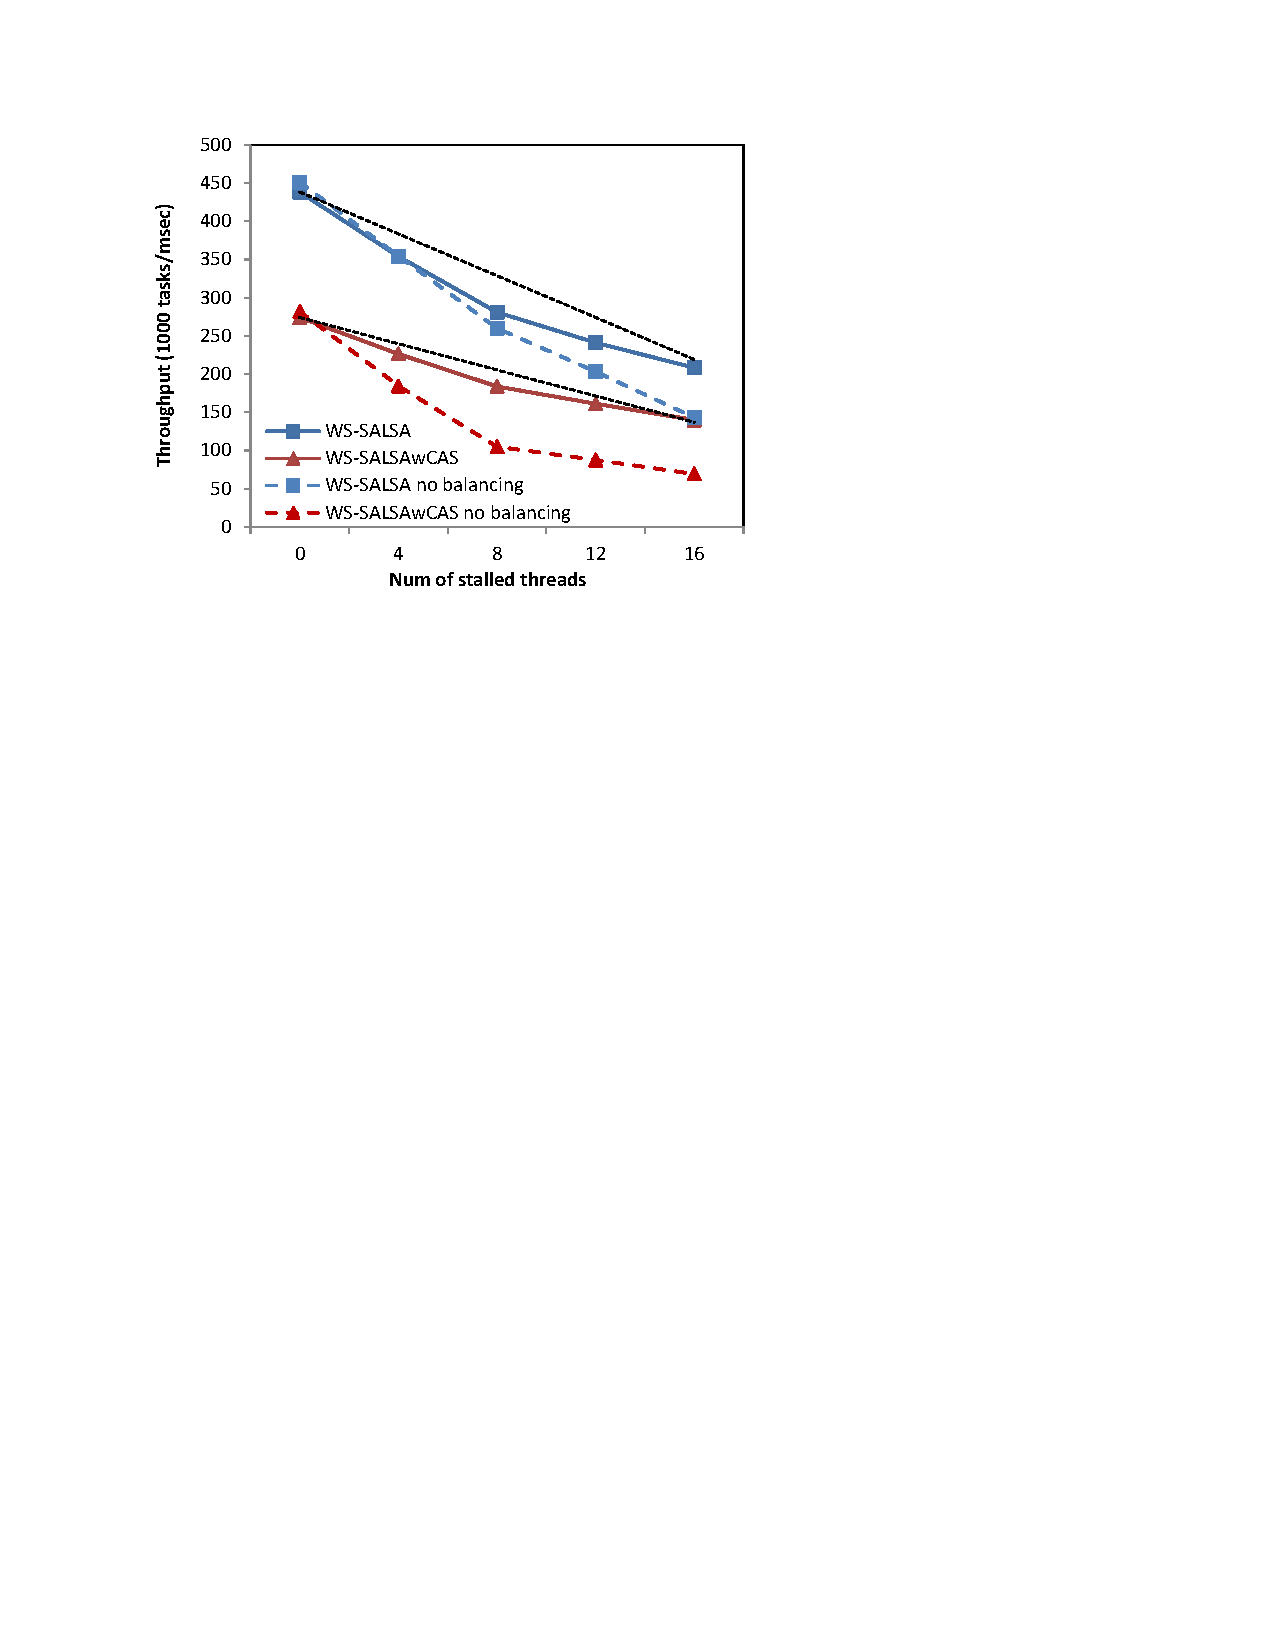
\includegraphics[width=0.45\textwidth]{figures/stalled-threads}
%  \end{center}
%  \vspace{-20pt}
%  \caption{\footnotesize{System throughput in a system with $16$ producers and $16$ consumers as a function of the number of stalled threads.}}
%  \vspace{-10pt}
%  \label{fig:stalled-threads}
%\end{wrapfigure}
%
%%
%%
%%\begin{figure}[htb]
%%	\centering
%%	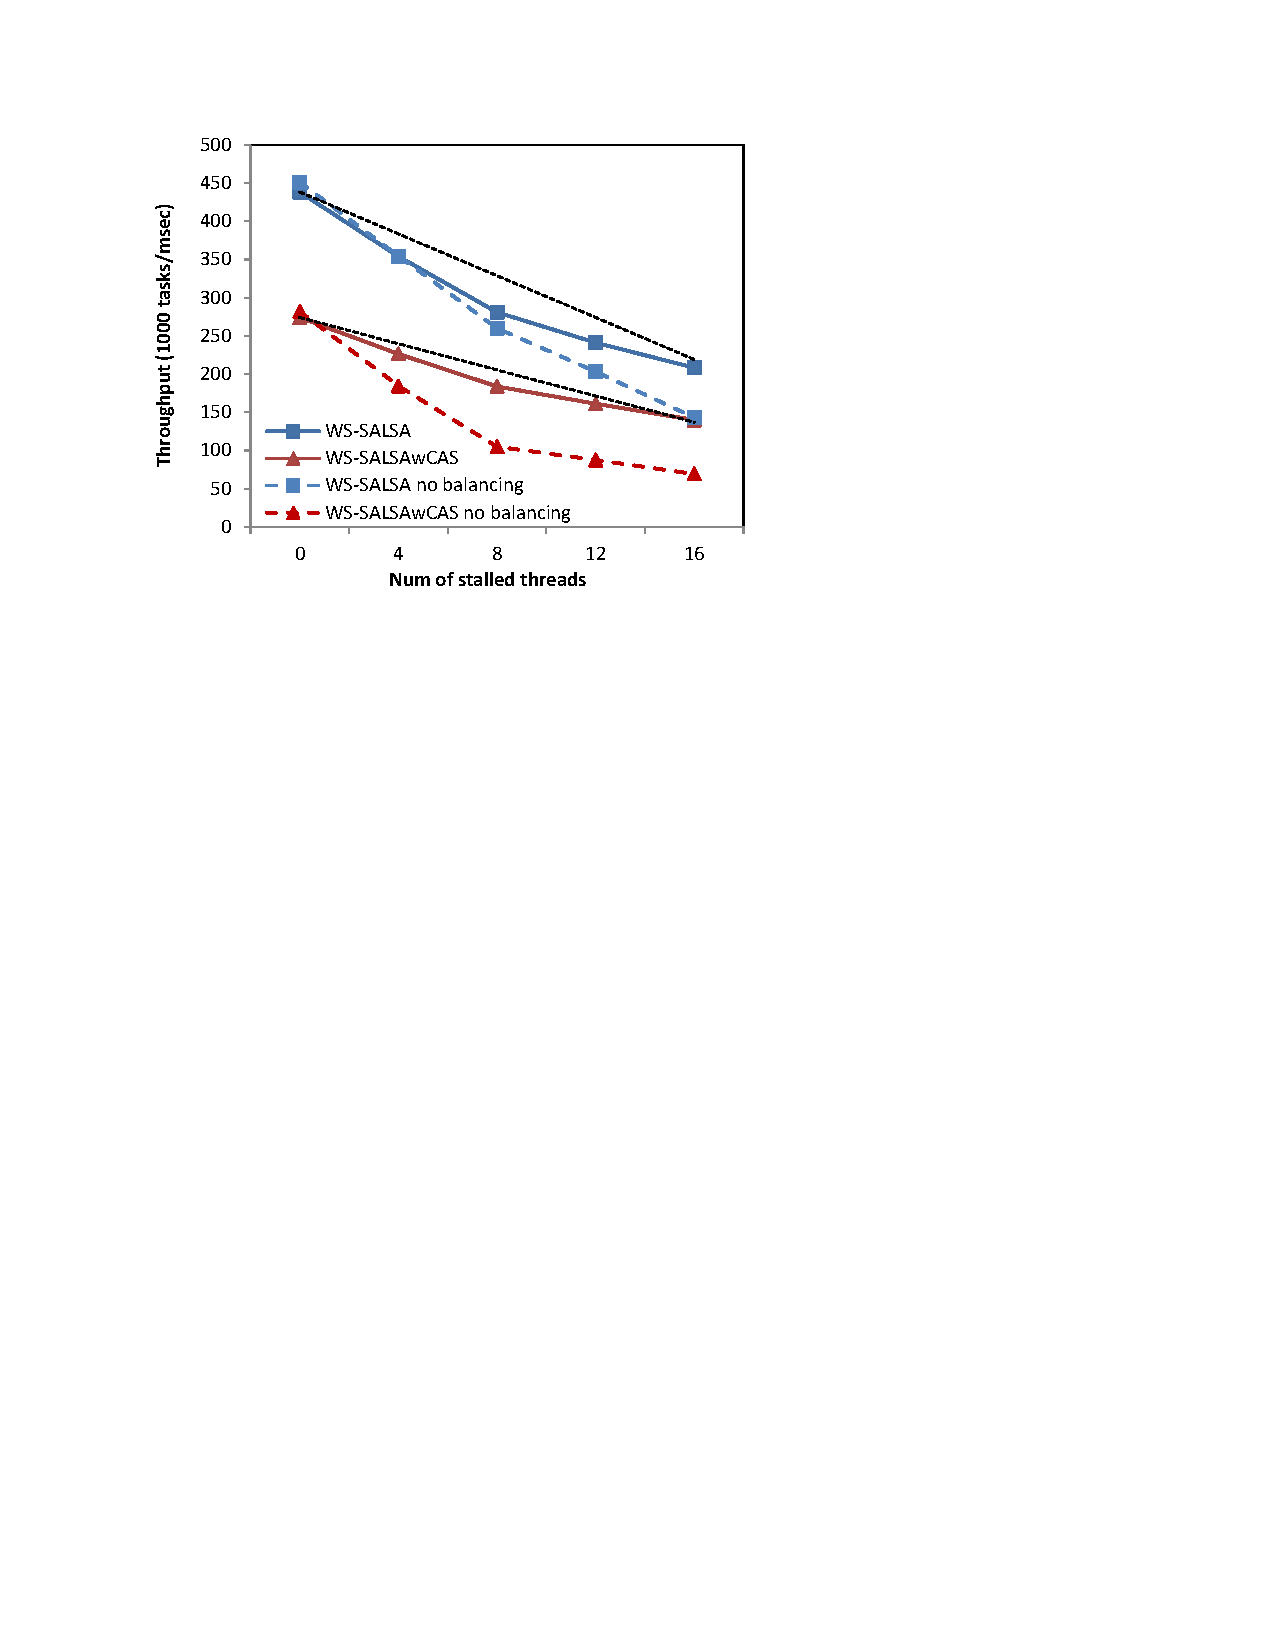
\includegraphics[width=0.45\textwidth]{figures/stalled-threads}
%%  \caption{\footnotesize{System throughput for different number of stalled threads (N/N workload). }}
%%	\label{fig:stalled-threads}
%%\end{figure}
%
%producer migration -- robustness against unpredictable stalls
%
%\begin{figure}[htb]
%	\centering
%	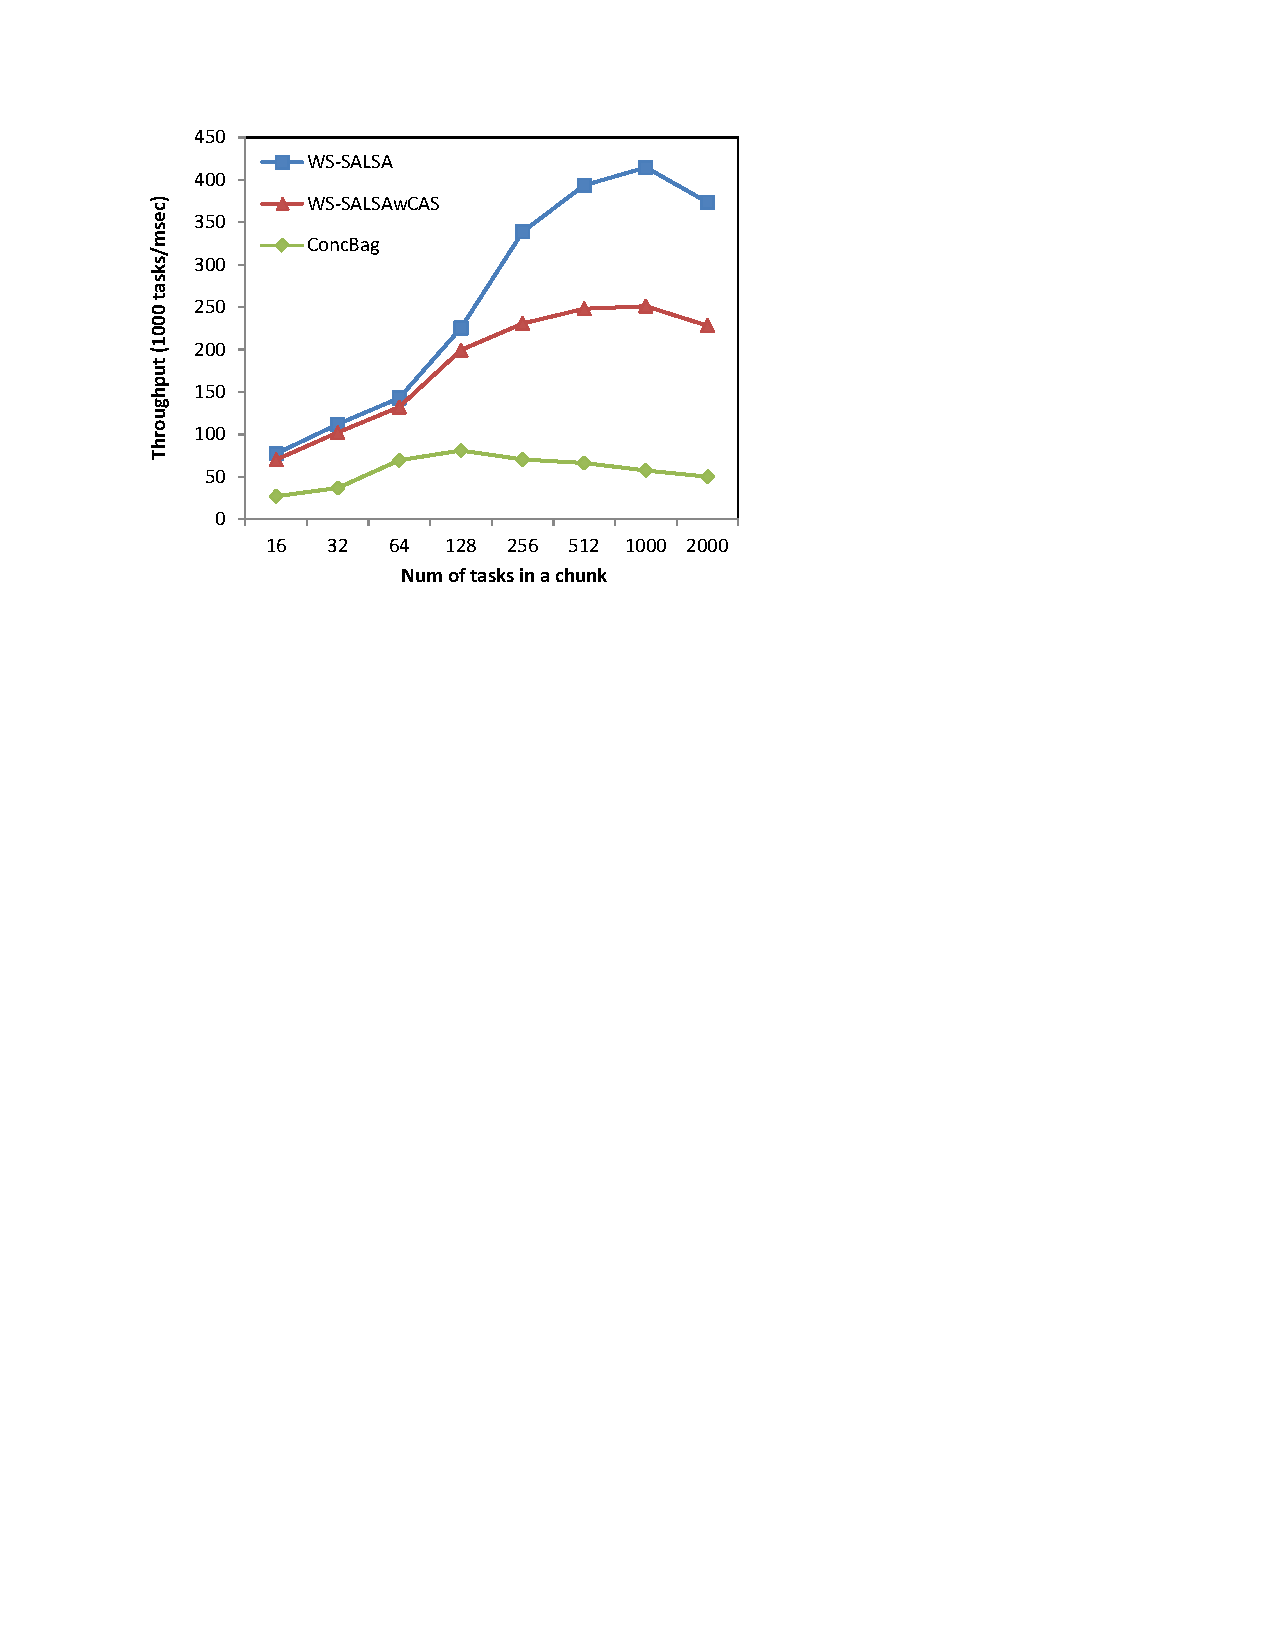
\includegraphics[width=0.45\textwidth]{figures/chunk-size}
%  \caption{\footnotesize{System throughput as a function of chunk size. }}
%	\label{fig:chunk-size}
%\end{figure}